% !TeX spellcheck = en_US
\documentclass[conference]{IEEEtran}
\IEEEoverridecommandlockouts
% The preceding line is only needed to identify funding in the first footnote. If that is unneeded, please comment it out.
\usepackage{cite}
\usepackage{amsmath,amssymb,amsfonts}
\usepackage{algorithmic}
\usepackage{graphicx}
\usepackage{textcomp}
\usepackage{xcolor}
\def\BibTeX{{\rm B\kern-.05em{\sc i\kern-.025em b}\kern-.08em
    T\kern-.1667em\lower.7ex\hbox{E}\kern-.125emX}}
\begin{document}

\title{Wireless smart monitoring energy system: a proof of concept}
{
%\thanks{Identify applicable funding agency here. If none, delete this.}
}

\author{
\IEEEauthorblockN{Marco Costantino}
\IEEEauthorblockA{\textit{Department of Mathematics} \\
\textit{University of Padova}\\
Padova, Italy \\
marco.costantino@studenti.unipd.it}
\and
\IEEEauthorblockN{Francesco Magarotto}
\IEEEauthorblockA{\textit{Department of Mathematics} \\
\textit{University of Padova}\\
Padova, Italy \\
francesco.magarotto@studenti.unipd.it}
}

\maketitle

\begin{abstract}
This document describes a prototype of domotic smart plugs. The system developed includes the smart plugs, a server, and a web interface that allow the user to monitor the power consumption of each individual appliance connected and power them on and off remotely. Furthermore, the system, provided that its settings are correct, keeps the user from turning on enough appliances to trigger the circuit breaker. The prototype has been developed keeping in mind issues of power consumption and reliability of communication between components of the system while keeping the traffic light.
\end{abstract}

\begin{IEEEkeywords}
Domotic plugs; Reliable UDP;
\end{IEEEkeywords}

\section{Introduction}
Nowadays, keeping track of domestic energy usage is a common scenario in domotic applications that aim to monitor the real-time watt consumption of home appliances. In most cases, the solution is a sensor connected to the main safety switch yielding the total energy consumption. Our approach, to get more detailed information and to have control over the use of power by the appliances, is to have an energy sensor for each plug connected to the 220V line. In the following paragraphs, we present our \textit{proof of concept} (POC) which, functionally, consists of three main components: the smart plugs, the server, and the web interface. In our POC, we have modified the architecture described in \cite{8110428} obtaining a specific low-energy consumption-driven infrastructure. This consists of the smart plugs, a computer (for the server), and a device (for the web interface). In a home scenario, these devices are connected to the home wireless router. The communication between smart plugs and server occurs over UDP with a simple form of reliability implemented at the application level and tested using Wireshark \cite{wireshark}. The architecture implemented differs from the most common ones in two major aspects: first, most homes aren't equipped with this kind of system, instead, a circuit breaker triggers for safety reasons when too much power is being consumed. Second, when a similar system is used it usually relies on cloud computing or external services. In contrast, our system offers the functionalities already described and both computing and data storage are performed locally. This can be an advantage in terms of both privacy and security. Furthermore, this is an advantage in terms of reliability: our system doesn't need an internet connection to work properly, instead, it just needs a working WLAN. However, while this aspect is significant, the development of the prototype hasn't focused on the security aspects and some issues will be discussed in the appropriate section. The architecture of the system is such that if need be it can be easily modified to use third-party services. The smart plugs have been prototyped using Arduino and the server has been written in Java. Let's now consider a use case example: the user sets the maximum power consumption possible in the home and then turns on two appliances. When this happens for the first time the system decides, based on the type of appliance connected, a default value for the maximum power usage of the appliance. This value is then updated to reflect the real maximum power usage of the appliance. Now that the system is running and some appliances are turned on, the user will be able to switch on only the appliances that consume less than the available power. Our POC covers this use case and shows that such a system can be practical and useful and that the traffic generated isn't enough to sensibly worsen the performances of the typical home WLAN. To summarize, the system keeps the power usage from reaching the maximum limit set by the user by forbidding the power-on of appliances that consume more than the available power. It also gives granular information about the energy consumption of the device and allows the user to turn on or off appliances remotely (via web interface). Aside from the main use case, in the age of climate awareness, such a system could be interesting to an environmentally conscious user that can monitor the power usage of appliances but also could set the maximum power consumption to be lower than the real one to use less power or save money. 

\section{General architecture}
The general architecture has 3 main components: the smart plugs, the server, and the web interface. The smart plugs have been prototyped using Arduino. The server has been developed in Java and the web interface is written in React. The rundown of what each part does is as follows: Arduino drives a sensor that gathers data on the power consumption of the plug and communicates with the UDP server that keeps track of the plugs and their energy consumption. The web interface uses an API exposed by the server to let the user see and control the status of each plug.
\begin{figure}[htbp]
	\centering
	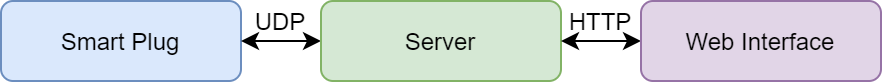
\includegraphics[width=\linewidth]{assets/architecture_schema}
	\caption{General architecture of the system}
	\label{fig:architecture_schema}
\end{figure}

\subsection{Smart plugs}\label{SP}
The smart plug is a small power plug which consists of a WeMos D1 R2 board, a 220v relay that can be controlled using 5 volts digital signals, and a coil connected to a PZEM-004T sensor which provides the readings to WeMos through its digital pins.
The connection scheme is represented in Figure~\ref{fig:pcbschema}, and has a cost about €25, so it is not so expensive. 
The WeMos D1 R2 board is equipped with a EPS 8266 wireless module operating at 2.4GHz. The connection settings are hardcoded in the software because storing it would require an SD module and an SD card. The board is programmed in C/C++ using Arduino IDE and uses the JSON format to serialize the data that will be sent, using a UDP library, to the server.
In every Arduino-like board, there is a function which allows our program to wait for UDP package arrivals from the server, affecting the relay status.
Another thread, once the board has recognized and registered the server, sends updates periodically if there is a variation greater than the 10\% of the energy consumption.
First, smart plugs wait for an \textit{INIT message}, sent by the server via broadcast. Once the packet has been received, each plug saves the information about the server and is not replying to this type of messages for a certain amount of type, or until a hard reset is performed. 
Then, the plug starts to send \textit{UPDATE messages} to inform the server about energy consumption variation. To do so, a thread keeps watch over the readings provided by the PZEM sensor.
In order to switch correctly the relay, the board waits for \textit{ON/OFF messages} from the server. After those requests have been received correctly, the correct action is performed and then an \textit{ACK message} is sent to inform the server about the successful receipt of the command.
\begin{figure}[htbp]
	\centering
	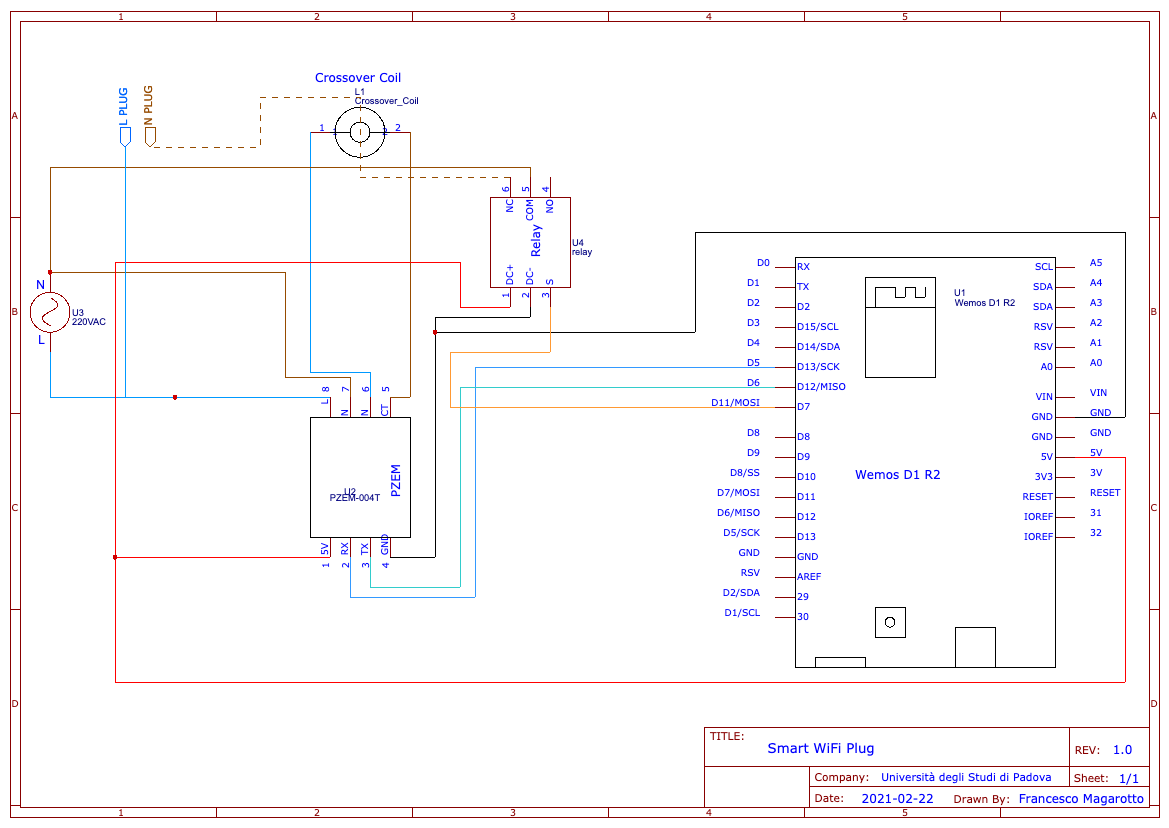
\includegraphics[width=\linewidth]{assets/pcb_schema}
	\caption{Electric schema of the wireless smart plug}
	\label{fig:pcbschema}
\end{figure}

\subsection{Server}\label{SVR}
The server has been developed in Java 8 and managed using Maven. Tomcat is implemented to expose the servlet API. The server has the following responsibilities:
\begin{itemize}
	\item It periodically broadcasts \textit{INIT messages} to let the plugs know its address;
	\item It listens for connections and updates from the plugs;
	\item It waits for acknowledgments from the plugs and, in case they are not received, it retransmits the lost packets;
	\item It exposes servlets to let the web interface get information about the plugs and send \textit{ON/OFF messages}.
\end{itemize}
The periodic actions, namely, sending the \textit{INIT message} and retransmitting those that are lost, are implemented as extensions of \textit{Guava's AbstractScheduledService} which allows performing of these at constant intervals. Another thread waits and manages the plugs' responses. When a plug responds to the \textit{INIT message} the server will register its information and estimate the max power consumption for the appliance connected to the plug. This value is simply based on average values for the given appliance type as found on Google. When a plug sends an \textit{UPDATE message} the server will update its registered information, most important: the current energy consumption and the max energy consumption. Finally, the server waits for the acknowledgments of previously sent messages. These messages are kept with a timestamp until an acknowledgment with the same timestamp is received. If a configurable number of seconds elapses before this happens the packet will be sent again. The servlets simply allow the web interface to get the server's information about the plugs (the type of appliance connected, the current energy consumption, and more) and to turn ON or OFF any given plug. In this last case, a packet will be sent by the server and for it the server will wait for an acknowledgment. The information about the plugs saved by the server is kept as a \textit{thread-safe hashmap}. Some of this information, such as the IP address of the plugs, the type of appliance connected and the max power consumption is also saved in a \textit{XML file} to avoid loosing it in case of a server malfunction or restart.
\subsection{Web interface}\label{WI}
The web interface is written in React using Bootstrap and exposes a way to interact with the server to get 
the real-time power consumption for each plug and managing the connected devices. It performs some to HTTP, so over TCP, to the API exposed by the server through the servlet, performing polling calls. The GUI shown in Figure \textbf{put figure here} presents a switch where the user can turn on or off the plug. If there is not enough energy available to turn on a device, the switch will be displayed as disabled in order to avoid a blackout.
\section{System results}
\section{Consumption}
%Qui mettiamo workflow generale con immagine algoritmo 


%
%\subsection{Maintaining the Integrity of the Specifications}
%
%The IEEEtran class file is used to format your paper and style the text. All margins, 
%column widths, line spaces, and text fonts are prescribed; please do not 
%alter them. You may note peculiarities. For example, the head margin
%measures proportionately more than is customary. This measurement 
%and others are deliberate, using specifications that anticipate your paper 
%as one part of the entire proceedings, and not as an independent document. 
%Please do not revise any of the current designations.
%
%\section{Prepare Your Paper Before Styling}
%Before you begin to format your paper, first write and save the content as a 
%separate text file. Complete all content and organizational editing before 
%formatting. Please note sections \ref{AA}--\ref{SCM} below for more information on 
%proofreading, spelling and grammar.
%
%Keep your text and graphic files separate until after the text has been 
%formatted and styled. Do not number text heads---{\LaTeX} will do that 
%for you.
%
%\subsection{Abbreviations and Acronyms}\label{AA}
%Define abbreviations and acronyms the first time they are used in the text, 
%even after they have been defined in the abstract. Abbreviations such as 
%IEEE, SI, MKS, CGS, ac, dc, and rms do not have to be defined. Do not use 
%abbreviations in the title or heads unless they are unavoidable.
%
%\subsection{Units}
%\begin{itemize}
%\item Use either SI (MKS) or CGS as primary units. (SI units are encouraged.) English units may be used as secondary units (in parentheses). An exception would be the use of English units as identifiers in trade, such as ``3.5-inch disk drive''.
%\item Avoid combining SI and CGS units, such as current in amperes and magnetic field in oersteds. This often leads to confusion because equations do not balance dimensionally. If you must use mixed units, clearly state the units for each quantity that you use in an equation.
%\item Do not mix complete spellings and abbreviations of units: ``Wb/m\textsuperscript{2}'' or ``webers per square meter'', not ``webers/m\textsuperscript{2}''. Spell out units when they appear in text: ``. . . a few henries'', not ``. . . a few H''.
%\item Use a zero before decimal points: ``0.25'', not ``.25''. Use ``cm\textsuperscript{3}'', not ``cc''.)
%\end{itemize}
%
%\subsection{Equations}
%Number equations consecutively. To make your 
%equations more compact, you may use the solidus (~/~), the exp function, or 
%appropriate exponents. Italicize Roman symbols for quantities and variables, 
%but not Greek symbols. Use a long dash rather than a hyphen for a minus 
%sign. Punctuate equations with commas or periods when they are part of a 
%sentence, as in:
%\begin{equation}
%a+b=\gamma\label{eq}
%\end{equation}
%
%Be sure that the 
%symbols in your equation have been defined before or immediately following 
%the equation. Use ``\eqref{eq}'', not ``Eq.~\eqref{eq}'' or ``equation \eqref{eq}'', except at 
%the beginning of a sentence: ``Equation \eqref{eq} is . . .''
%
%\subsection{\LaTeX-Specific Advice}
%
%Please use ``soft'' (e.g., \verb|\eqref{Eq}|) cross references instead
%of ``hard'' references (e.g., \verb|(1)|). That will make it possible
%to combine sections, add equations, or change the order of figures or
%citations without having to go through the file line by line.
%
%Please don't use the \verb|{eqnarray}| equation environment. Use
%\verb|{align}| or \verb|{IEEEeqnarray}| instead. The \verb|{eqnarray}|
%environment leaves unsightly spaces around relation symbols.
%
%Please note that the \verb|{subequations}| environment in {\LaTeX}
%will increment the main equation counter even when there are no
%equation numbers displayed. If you forget that, you might write an
%article in which the equation numbers skip from (17) to (20), causing
%the copy editors to wonder if you've discovered a new method of
%counting.
%
%{\BibTeX} does not work by magic. It doesn't get the bibliographic
%data from thin air but from .bib files. If you use {\BibTeX} to produce a
%bibliography you must send the .bib files. 
%
%{\LaTeX} can't read your mind. If you assign the same label to a
%subsubsection and a table, you might find that Table I has been cross
%referenced as Table IV-B3. 
%
%{\LaTeX} does not have precognitive abilities. If you put a
%\verb|\label| command before the command that updates the counter it's
%supposed to be using, the label will pick up the last counter to be
%cross referenced instead. In particular, a \verb|\label| command
%should not go before the caption of a figure or a table.
%
%Do not use \verb|\nonumber| inside the \verb|{array}| environment. It
%will not stop equation numbers inside \verb|{array}| (there won't be
%any anyway) and it might stop a wanted equation number in the
%surrounding equation.
%
%\subsection{Some Common Mistakes}\label{SCM}
%\begin{itemize}
%\item The word ``data'' is plural, not singular.
%\item The subscript for the permeability of vacuum $\mu_{0}$, and other common scientific constants, is zero with subscript formatting, not a lowercase letter ``o''.
%\item In American English, commas, semicolons, periods, question and exclamation marks are located within quotation marks only when a complete thought or name is cited, such as a title or full quotation. When quotation marks are used, instead of a bold or italic typeface, to highlight a word or phrase, punctuation should appear outside of the quotation marks. A parenthetical phrase or statement at the end of a sentence is punctuated outside of the closing parenthesis (like this). (A parenthetical sentence is punctuated within the parentheses.)
%\item A graph within a graph is an ``inset'', not an ``insert''. The word alternatively is preferred to the word ``alternately'' (unless you really mean something that alternates).
%\item Do not use the word ``essentially'' to mean ``approximately'' or ``effectively''.
%\item In your paper title, if the words ``that uses'' can accurately replace the word ``using'', capitalize the ``u''; if not, keep using lower-cased.
%\item Be aware of the different meanings of the homophones ``affect'' and ``effect'', ``complement'' and ``compliment'', ``discreet'' and ``discrete'', ``principal'' and ``principle''.
%\item Do not confuse ``imply'' and ``infer''.
%\item The prefix ``non'' is not a word; it should be joined to the word it modifies, usually without a hyphen.
%\item There is no period after the ``et'' in the Latin abbreviation ``et al.''.
%\item The abbreviation ``i.e.'' means ``that is'', and the abbreviation ``e.g.'' means ``for example''.
%\end{itemize}
%An excellent style manual for science writers is \cite{b7}.
%
%\subsection{Authors and Affiliations}
%\textbf{The class file is designed for, but not limited to, six authors.} A 
%minimum of one author is required for all conference articles. Author names 
%should be listed starting from left to right and then moving down to the 
%next line. This is the author sequence that will be used in future citations 
%and by indexing services. Names should not be listed in columns nor group by 
%affiliation. Please keep your affiliations as succinct as possible (for 
%example, do not differentiate among departments of the same organization).
%
%\subsection{Identify the Headings}
%Headings, or heads, are organizational devices that guide the reader through 
%your paper. There are two types: component heads and text heads.
%
%Component heads identify the different components of your paper and are not 
%topically subordinate to each other. Examples include Acknowledgments and 
%References and, for these, the correct style to use is ``Heading 5''. Use 
%``figure caption'' for your Figure captions, and ``table head'' for your 
%table title. Run-in heads, such as ``Abstract'', will require you to apply a 
%style (in this case, italic) in addition to the style provided by the drop 
%down menu to differentiate the head from the text.
%
%Text heads organize the topics on a relational, hierarchical basis. For 
%example, the paper title is the primary text head because all subsequent 
%material relates and elaborates on this one topic. If there are two or more 
%sub-topics, the next level head (uppercase Roman numerals) should be used 
%and, conversely, if there are not at least two sub-topics, then no subheads 
%should be introduced.
%
%\subsection{Figures and Tables}
%\paragraph{Positioning Figures and Tables} Place figures and tables at the top and 
%bottom of columns. Avoid placing them in the middle of columns. Large 
%figures and tables may span across both columns. Figure captions should be 
%below the figures; table heads should appear above the tables. Insert 
%figures and tables after they are cited in the text. Use the abbreviation 
%``Fig.~\ref{fig}'', even at the beginning of a sentence.
%
%\begin{table}[htbp]
%\caption{Table Type Styles}
%\begin{center}
%\begin{tabular}{|c|c|c|c|}
%\hline
%\textbf{Table}&\multicolumn{3}{|c|}{\textbf{Table Column Head}} \\
%\cline{2-4} 
%\textbf{Head} & \textbf{\textit{Table column subhead}}& \textbf{\textit{Subhead}}& \textbf{\textit{Subhead}} \\
%\hline
%copy& More table copy$^{\mathrm{a}}$& &  \\
%\hline
%\multicolumn{4}{l}{$^{\mathrm{a}}$Sample of a Table footnote.}
%\end{tabular}
%\label{tab1}
%\end{center}
%\end{table}
%
%\begin{figure}[htbp]
%\centerline{
\includegraphics{fig1.png}}
%\caption{Example of a figure caption.}
%\label{fig}
%\end{figure}
%
%Figure Labels: Use 8 point Times New Roman for Figure labels. Use words 
%rather than symbols or abbreviations when writing Figure axis labels to 
%avoid confusing the reader. As an example, write the quantity 
%``Magnetization'', or ``Magnetization, M'', not just ``M''. If including 
%units in the label, present them within parentheses. Do not label axes only 
%with units. In the example, write ``Magnetization (A/m)'' or ``Magnetization 
%\{A[m(1)]\}'', not just ``A/m''. Do not label axes with a ratio of 
%quantities and units. For example, write ``Temperature (K)'', not 
%``Temperature/K''.
%
%\section*{Acknowledgment}
%
%The preferred spelling of the word ``acknowledgment'' in America is without 
%an ``e'' after the ``g''. Avoid the stilted expression ``one of us (R. B. 
%G.) thanks $\ldots$''. Instead, try ``R. B. G. thanks$\ldots$''. Put sponsor 
%acknowledgments in the unnumbered footnote on the first page.

\bibliography{references.bib}{}
\bibliographystyle{IEEEtran}

\end{document}
